%\RequirePackage[l2tabu, orthodox]{nag}

\documentclass[11pt,oneside]{report}
\usepackage[a4paper, margin=1.5in]{geometry}
%\usepackage{fullpage}
\usepackage{url}
\usepackage{graphicx}
\usepackage{harvard}
\usepackage{mathtools}
\usepackage{parskip}
\usepackage{subcaption}
\usepackage{bashful}
\usepackage{microtype}
\usepackage{float}
\usepackage{hyperref}
\usepackage{fancyhdr}
\usepackage[font={small,it}]{caption}

\pagestyle{fancy}
\fancyhf{}
\rhead{\thepage}
\lhead{\leftmark}
\cfoot{}

\citationmode{abbr}
\renewcommand{\baselinestretch}{1.5}
%\renewcommand{\familydefault}{\sfdefault}

\graphicspath{{images/}}

\title{An Open Source Computer Vision Library for Leapmotion}
\author{Daniel Hamilton 10026535,\\Computer Science,\\University of the West of England.}
	
\bash
texcount -sum -1 report.tex
\END

\begin{document}
	\maketitle
	\tableofcontents

	
	Word Count: \bashStdout.
	\begin{abstract}
	
	\end{abstract}	
	%----------------------------------------- Chapter 1 -----------------------------------------%
	\chapter{Introduction}\label{chap:introduction}
		\section{Computer Vision: An Intellectual Frontier}
			\subsection{What is Computer Vision?}		
				
				It is very hard for humans to know what their own biological vision really entails, and how difficult it is to reproduce on a computer.
				Information from the eyes is divided into multiple channels, each streaming different kinds of information to the brain.
				The brain then subconsciously groups and identifies the parts of the image to examine along with what parts to suppress.
				The way in which biological vision works is still largely unknown which makes it hard to emulate on computers \cite[p. xi]{book:multiViewGeo}.				
				Computer vision systems are still relatively naive, all they "see" is a grid of numbers.%from def:cv
				
				%By default there is no built in pattern recognition, or what some might call, intelligence.
				
				Computer vision is a vast field and hard to define.
				For the purpose of this report it will be defined as:
	
				\begin{quote}
					``\textit{The transformation of data from a still or video camera into either a decision or a new representation.
						All transformations are done for achieving some particular goal.}'' \cite[p. 2]{definition:cv}
				\end{quote}
				
				Even though computer vision in terms of comparison to biological vision, still remains an unsolved problem, there have still been many excellent achievements in the field to date.
			\subsection{Uses of Computer Vision}
				One of the most prominent uses of computer vision currently, is in driver less cars.
				Which in recent years, have reached a level of sophistication at which they are being approved by governments to be used on public highways \cite{web:driverlessCars}.
				Complex and expensive equipment with the capability to analyse a three-dimensional scene in real-time is required to achieve this.
				%Add the http://velodynelidar.com/lidar/hdlproducts/hdl64e.aspx here, try and find a price to reference "expensive" maybe mention google explicitely.
				Computer vision is also used on manufacturing production lines.
				\citeasnoun{journal:salmon} set out to try and classify salmon fillets, to see if it was possible to determine whether a salmon fillet had been processed using enzymes. %maybe expand on what they actually did experementally here.
				However, computer vision isn't only available to big companies with large amounts of money to spend on research.
				\begin{quote}
				``\textit{Computer vision is a rapidly growing field, partly as a result of both cheaper and more capable cameras, partly because of affordable processing power, and partly because vision algorithms are starting to mature.}''\cite[p. ix]{definition:cv}
				\end{quote}
				One such device that has been made available is the Kinect by Microsoft.
				The computer vision society found that the capabilities of the Kinect could be extended beyond its intentional use for gaming, and at a much lower cost than traditional three dimensional cameras.
				It has been used in areas such as human activity analysis, where it is able to estimate details about the pose of the human subject in its field of vision \cite{kinect:1}.
				It has also been used to for real time odometry whilst attached to a quadcopter, enabling the production of a three dimensional mapping of a physical space \cite{kinect:2}.
				%The line below is dependant on a reference
				A hacking culture has enabled this type of exploitation of technology to take place and is spurring the creators of these technologies to make them more open.
				
			\subsection{OpenCV}
			
			%Introduction to OpenCV here. Overview, not in depth.	
				OpenCV is an open source computer vision library.
				It was designed for computational efficiency with a strong focus on real-time applications.
				One of OpenCV's goals is to provide a simple-to-use computer vision infrastructure that helps people build fairly sophisticated vision applications quickly \cite[p. 1]{definition:cv}.	
				It aimed to advance computer vision research by providing open and already optimised code.
				Providing a basic vision infrastructure with no need to reinvent the wheel.
				It also provided a common infrastructure on which knowledge of computer vision could be shared between developers.
				Making code more readable and transferable \cite[p. 6]{definition:cv}. 
				This is an overview for now but more specifics will be covered later in the document.
				
		\section{The Leap Motion Controller}
			\subsection{What is the Leap Motion?}
				%cite leapmotion https://developer.leapmotion.com/articles/intro-to-motion-control
				The Leap Motion Controller is a device aimed at providing a Natural User Interface through hand gestures.
				It is made up of two infra red cameras both with a fisheye lense, set up stereoscopically. %IMAGES OF CAMERA IN INFRA RED TO SHOW CAMERAS
				It provides functionality out of the box that allows a developer to track movements and gestures made by a hand \cite{web:leapGestures}.
				%Don't really need the price...
				It is discrete in size and has an accessible price. %maybe include the price here
				Leap motion have recently released a new version of their SDK, allowing access to more elements of their Leap Motion Controller. 
				Namely, images from the two cameras. 
				This allows the library user to generate a three dimensional representation of a scene, using techniques of which are discussed later in this document. %define disparity
				The source code for the SDK is closed source, therefore it is not known the current methods by which hands and gestures are classified \cite[p. 217]{journal:leapEvaluation}.
				With the access to the images it allows exploration of other, custom methods for classification.

			\subsection{Uses in Computer Vision}
				The Leap Motion Controller has already been used in many innovative ways.
				An example being its use in recognising Australian and Arabic sign language \cite{journal:leapSignLanguage,journal:leapSignLanguage2}.
				However these solutions only make use of the default detection system in the SDK.
				While these are useful, raw image access is required to detect other types of object.
				Now that this capability has been made available however, a whole new future of possibilities have been opened.
				Having access to the images allows for their use in computer vision.
				In turn this means that such an accessible and small device can be used in a variety of new ways.
				By creating an open source computer vision library for the leap motion, it might become of use in the field of robotics.
				It's size would make it suitable for much smaller robots.
				%need to talk about its use in areas such as robotic arms to pick up things for packaging etc.
				
		\section{Product Expectations}
		%define the boundaries of the project		
		
	%----------------------------------------- Chapter 2 -----------------------------------------%
	\chapter{Background Research}\label{chap:background}
		\section{Literature Review}
			\subsection{Stereopsis and Calibration}
			\begin{quote}
				``\textit{Stereo matching is the process of taking two or more images and estimating a 3D model of the scene by finding matching pixels in the images and converting their 2D positions into 3D depths.}''\cite{book:sam}
			\end{quote}
			The idea behind this stems from the way that biological vision works.
			In humans, depth is perceived from the difference between the images produced by the left and the right eye.
			%cite some stuff about algorithm performance from the scelzki2002aa paper
			To emulate this in computer vision, the images of a scene produced by the cameras are taken from two different positions.
			One of the difficulties then faced with stereo matching is being able to identify the corresponding pixels in each image taken.
			When using two cameras, as those that are to be provided by the Leap Motion, \citeasnoun[p. 415]{definition:cv} define four steps that are needed to achieve successful correspondence between the images produced by each.
			
			\begin{enumerate}
				%CHECK THESE ARE CORRECT
				\item Mathematically remove radial and tangential lense distortion; this is called undistortion. The outputs to this step are undistorted images.
				
				\item Adjust for the angles and distances between cameras, a process called rectification. The outputs of this step are images that are row-aligned and rectified.
				
				\item Find the same features in the left and right camera views, a process known as correspondence. The output of this step is a disparity map, where the disparities are the differences in $x$-coordinates on the image planes of the same feature viewed in the left and right cameras: $x^{l} - x^{r}$.
				
				\item If we know the geometric arrangement of the cameras, then we can turn the disparity map into distances by triangulation. This step is called reprojection, and the output is a depth map.
			\end{enumerate}
			
			For the system to make successful use of the images, it needs to know the set up of the cameras (calibration).
			%epipolar geometry
			Much research has already been done on this.
			As a result, computer vision libraries have appeared, such as OpenCV.
			Libraries like this create a layer of abstraction between the user and the underlying low-level image processing.
			Allowing the process of calibration to be carried out with ease, not needing to know all of the mathematics behind the process.
			Although it is good to have a general overview of what is happening.
			As this is a fundamental element to this project, each stage of calibration will be covered in a little more detail.
				\subsubsection{Image Correction}
				%get the fundamental matrix using opencv
				Images produced by cameras with lenses suffer from aberrations.
				No lens is perfect.
				Therefore correction is needed to get a true representation of the objects in the image.
				There are many different types of aberration, but the only one that will be discussed here is distortion.
				Distortion is an effect that changes the overall shape of an image (geometric warping) (See Figure \ref{distortion}).
				\begin{figure}[!h]
				\begin{center}
					
    					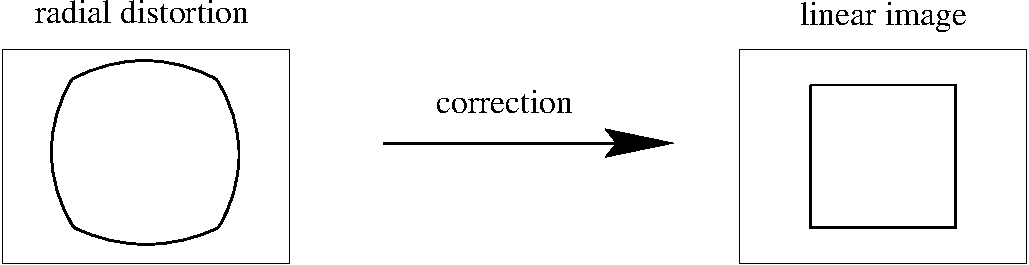
\includegraphics[scale=0.5]{distortion_1}
    					\caption{Example of radial distortion of a square being corrected \protect\cite{book:multiViewGeo} {\label{distortion}}}
    				\end{center}
				\end{figure}				
				It is caused by the fact that different areas of a lens have slightly different focal lengths \cite[p. 42]{book:modern}.
				There is a lot of information available on how distortion happens so only the basics will be covered here, however some reading suggestions are (READING SUGGESTIONS HERE).
				The fundamental stages of processing images for use in computer vision comes down to geometry.
				To reliably calculate depth in a scene, the system needs to know the intrinsic %and extrinsic 
				parameters of a camera.
				Essentially, the system wants to know if what the camera is producing is a true representation of the scene it is recording.
				Much like when you make a visit to see an optician. 
				The optician will carry out a process to try and discover if what you see is a distortion of reality.
				The parameters will allow the system to take the images and pre process them (undistort) so that it can be confident they are true.
				This is done by producing both a camera geometry and a lens distortion model through a process of calibration.  
				The two models will now be discussed in a little more depth.				
				%more depth here
				\subsubsection{Camera Model}
				Most of the information available on camera models are focused around a pinhole camera.
				The following description and figures of this model is taken from \citeasnoun[p. 371-373]{definition:cv}, If more depth is needed I advise you read the cited material.
				The pinhole camera model is the most basic type of camera, that still holds the fundamental mathematics on how most modern digital cameras work today.
				\begin{figure}[!ht]
				\begin{center}
					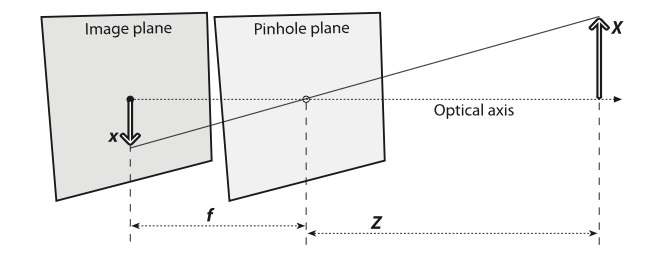
\includegraphics[scale=0.5]{pinhole}
					\caption{Pinhole camera model as shown in in \protect\citeasnoun[p. 372]{definition:cv} {\label{pinhole}}}
				\end{center}
				\end{figure}
				In a pinhole camera (See Figure \ref{pinhole}) light reflected from the scene/object travels through a pinhole that is made in the pinhole plane.
				This light then gets projected onto the image plane.
				The size of this projected image is proportional to the focal length $f$.
				Where $Z$ is the distance from the pinhole plane to the object, $X$ is the length of the object and $x$ is the objects image on the image plane.
				Therefore we can work out the size of the object using the equation $-x=f\dfrac{X}{Z}$.
				For mathematical simplification \citeasnoun{definition:cv} states that the negative value can be ommited leaving $x=f\dfrac{X}{Z}$.
				This is done by moving the image plane in front of the pinhole plane, and then treating the pinhole as a center of projection (See Figure \ref{pinhole2}).
				This gives us with an image that is the correct way up, although it would be impossible to make this camera physically.
				\begin{figure}[!ht]
				\begin{center}
					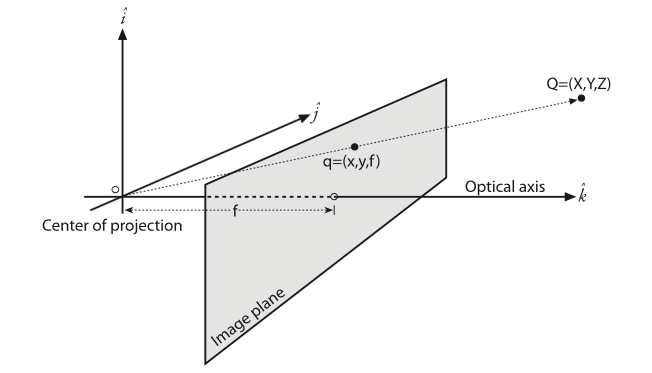
\includegraphics[scale=0.5]{pinhole2}
					\caption{Pinhole camera model with image plane in front, as shown in in \protect\citeasnoun[p. 372]{definition:cv} {\label{pinhole2}}}
				\end{center}
				\end{figure}
				%THIS ASSUMES KNOWLEDGE ON HOW A CAMERA WORKS
				In the real world, the center of projection will not be precisely in the middle of the imaging sensor of a camera.
				Therefore displacement values need to be considered, $c_{x}$ and $c_{y}$.
				The resulting model allows us to pinpoint the point $Q$ with coordinates $(X,Y,Z)$ as a pixel location given as $(x_{screen}, y_{screen})$.
				With the resulting mathematical model of $x_{screen}=f_{x}\left(\dfrac{X}{Z}\right)+c_{x}$, $y_{screen}=f_{y}\left(\dfrac{Y}{Z}\right)+c_{y}$.
				Having an accurate model like this allows us to define the parameters of the camera so that false transformations of light being collected from the physical world can be corrected.
				This is important for methods of image rectification which will be discussed later.
				\subsubsection{Lens Distortion}
					The camera models discussed assume that cameras produce images in which the straight lines represent the same straight lines that are in the scene.
					However as discussed earlier a lens is never perfect and so many will create a visible curvature in the projections of straight lines in an image.
					Unless this distortion is taken into account, it becomes impossible to create highly accurate photorealistic reconstructions.
					A phenomenon known as radial distortion produces a visible curvature on the straight lines that appear in the image.
					This is where pixels in the image are displaced away or towards the image centre by an amount proportional to their radial distance.
					These types of distortion are known as barrel and pincushion respectively.
					The Leap Motion has a radial distortion, more specifically it is known as a fisheye.
					The fisheye is a distortion where the image that is produced provides an near 180(degree) span side-to-side \cite{book:sam}.
					
				\subsubsection{Image Rectification}
				
				
				
			\subsection{Machine Learning}%possibly falls under classification
			\subsection{Classification}
			\subsection{Vision Libraries}
				\subsubsection{OpenCV}
				\subsubsection{Point Cloud Library}
				
	%----------------------------------------- Chapter 3 -----------------------------------------%
	\chapter{Requirements Analysis}\label{chap:req}
	This chapter attempts to lay out a set of requirements for the Library, from the point of view of the users.
	They will set out a contract between the users and the library developer as a means to show what the library is going to be and how the library developer is going to build it.
	They provide goals upon which a realistic scope for the project may be set and will also be the backbone of the tests that are to be written for \autoref{chap:test}.
	\begin{itemize}
		\item \textbf{Stakeholder identification}
		\item \textbf{Use case analysis}
		\item \textbf{Functional requirements}
		\item \textbf{Non-functional requirements}
		\item \textbf{Prioritisation}
	\end{itemize}
		\subsection{Stakeholder identification}
		\subsection{Use case analysis}
		\subsection{Functional requirements}
		\subsection{Non-functional requirements}
		\subsection{Prioritisation}
	
	%----------------------------------------- Chapter 4 -----------------------------------------%
	\chapter{Design}\label{chap:des}
	%----------------------------------------- Chapter 5 -----------------------------------------%
	\chapter{Implementation}\label{chap:imp}
	
	%----------------------------------------- Chapter 6 -----------------------------------------%
	\chapter{Test}\label{chap:test}
		%----------------------------------------- Chapter 7 -----------------------------------------%
	\chapter{Evaluation}\label{chap:eval}
	%----------------------------------------- Chapter 7 -----------------------------------------%
	\chapter{Conclusion}\label{chap:concl}

	\bibliographystyle{dcu}
	\bibliography{bibfile}
\end{document}
